\chapter{Iteracion 2: Primer prototipo de software} % (fold)
\label{cha:iteracion_2}

\section{Introduccion} % (fold)
\label{sec:introduccion}

% fue cuando empezamos a tirar fruta. habiendo elegido el microcontrolador empezamos a probar todas las funcionalidades: El adc, los contadores de eventos, el modulo serial. Despues arrancamos a diseñar el primer prototipo. Consideramos que segun los requerimientos tenia que se un sistema que ofrezca algun tipo de interfaz para que un usuario interactue con el, para que pueda configurarle los parametros segun lo que se quiere lograr.

En esta iteracion se realizo el primer prototipo de programa a embeber en el microcontrolador para cumplir con los requerimientos planteados. Los primeros pasos incluyeron programas de prueba para verificar el funcionamiento de los distintos modulos del microcontrolador a utilizar: El conversor analogico-digital, la ganancia programable, los contadores y el modulo serial. 

% section introduccion (end)

\section{Requerimientos de la iteración} % (fold)
\label{sec:requerimientos_de_la_iteracion}

De los requerimientos principales, surgen los siguientes requerimientos para el programa a embeber en el microcontrolador:

\begin{itemize}
\item El programa deberia utilizar el conversor del microcontrolador para transformar señales analogicas de fuentes externas a datos digitales
\item El programa deberia utilizar los contadores del microcontrolador para contar eventos de fuentes externas
\item El programa deberia utilizar el modulo serial UART y SMBus del microcontrolador para enviar los datos a otra placa o microprocesador
\item Para cada canal del conversor:
\begin{itemize}
\item El usuario deberia poder habilitar o inhabilitar el canal para la medicion
\item El usuario deberia poder configurar el modo de medicion (canal unico o diferencial). En caso de ser canal unico deberia especificarse un solo canal, y dos canales para modo diferencial.
\item El usuario deberia poder configurar un tiempo de intervalo entre cada medicion
\end{itemize}
\item Para cada contador:
\begin{itemize}
\item El usuario deberia poder habilitar o inhabilitar el conteo de eventos.
\end{itemize}
\item El usuario deberia poder elegir el protocolo serial para comunicarse con la placa o microprocesador externo que recibira los datos (UART o SMBus).

\end{itemize}


% section requerimientos_de_la_iteracion (end)

\section{Desarrollo} % (fold)
\label{sec:desarrollo}

En esta seccion elaboramos el proceso de desarrollo que se llevo a cabo para construir el software a embeber en el microcontrolador C8051F252\cite{c8051f352}. Es necesario que se tenga en cuenta que fueron necesarias dos iteraciones para llegar al prototipo final. En esta seccion cubrimos solo la primera. La segunda iteracion de software, que fue en la que se llego al programa final de la placa de adquisicion, se encuentra en el capitulo \ref{cha:iteracion_5}

\section{Diseño y modelos estaticos} % (fold)
\label{sec:diseno_y_modelos_estaticos}

Para poder describir el programa de manera grafica, utilizamos modelos del patron de diseño SysML 1.1. Aunque no usamos este patron de diseño para el programa, lo utilizamos en este informe para describirlo de una manera formal.

\subsection{Modelos estaticos} % (fold)
\label{sub:modelos_estaticos}

Como primera instancia, realizamos un diagrama de caso de uso para tener una idea de lo que se quiere lograr con el programa. Es necesario tener en cuenta que por las caracteristicas del microcontrolador, existen ciertas limitaciones que limitan el software. Estas limitaciones estan listadas en la seccion \ref{sub:seleccion}.

\begin{figure}[h]
  \centering
  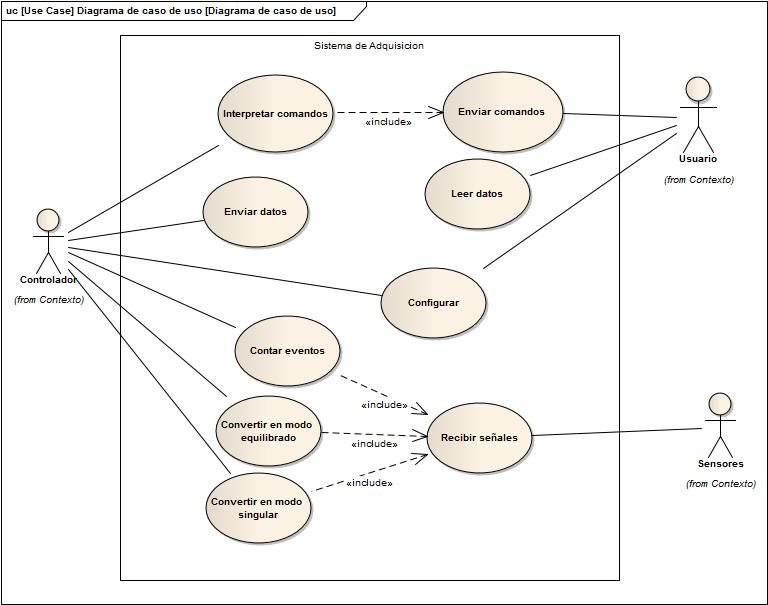
\includegraphics[width=0.80\textwidth, height = 11cm]{casouso1}
  \caption{Diagrama de caso de uso del sistema de medicion e instrumentacion}\label{fig:casouso1}
\end{figure}

El caso de uso ``configurar'' esta generalizado. Las acciones que incluye este caso son:
\begin{itemize}
  \item Configurar la interfaz serial
  \item Configurar canal en modo singular
  \item Configurar canal en modo equilibrado
  \item Configurar contador de eventos
  \item Configurar ganancia del del conversor
  \item Configurar intervalo de medicion para conversion analogica
\end{itemize}

\begin{figure}[h]
  \centering
  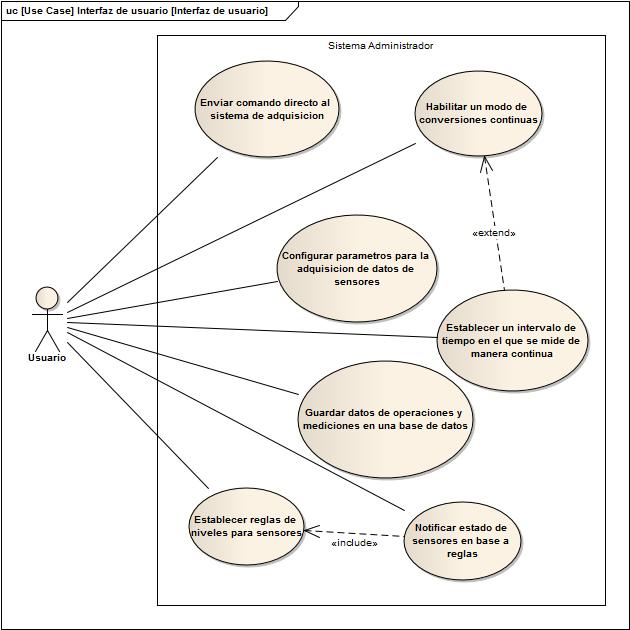
\includegraphics[width=0.80\textwidth, height = 11cm]{casousoAdministrador}
  \caption{Diagrama de caso de uso del sistema administrador}\label{fig:casousoAdministrador}
\end{figure}

En la figura \ref{fig:casouso1}, se puede ver el diagrama de caso de uso para el software a realizar. En cada caso de uso, pueden comenzar a visualizarse las distintas acciones que el programa debe realizar. Al no contar con la posibilidad de organizar el programa en clases, se separo en distintos modulos que agrupan funciones de caracteristicas similares. Estos modulos estan ilustrados como bloques en la figura \ref{fig:bloquesprimeraiteracionsoftware}. Cada bloque correponde a un modulo distinto dentro del programa. Se pueden ver los nombres de cada funcion y el tipo de retorno en cada uno de ellos. Con esto ultimo, damos una idea de las acciones realizadas por las funciones de cada modulo. Una descripcion mas detallada esta en la documentacion del programa \ref{documentacionsoftware}.

\begin{figure}[h]
  \centering
  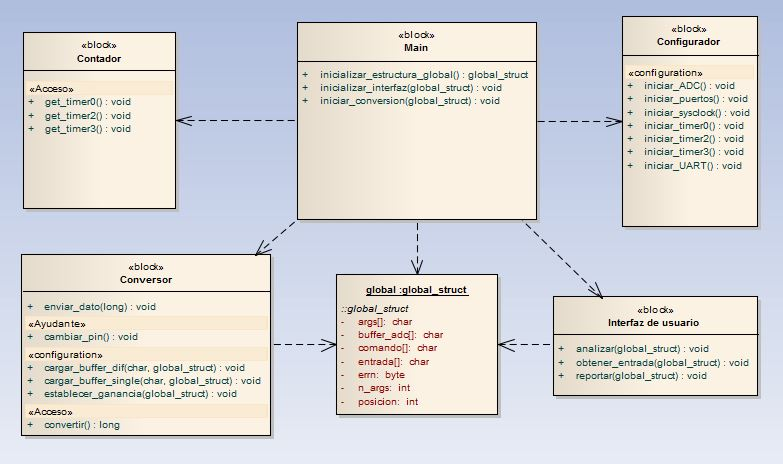
\includegraphics[width=0.80\textwidth, height = 11cm]{bloquesprimeraiteracionsoftware}
  \caption{Diagrama de bloques de la primera iteracion de software}\label{fig:bloquesprimeraiteracionsoftware}
\end{figure}

El objetivo de los diagramas ilustrados es una descripcion grafica del sistema. Es necesario destacar que, desde el principio, la evolucion del programa ocasiono que los diseños de los modulos fueran cambiando. Los cambios fueron debidos a multiples razones: particularidades del funcionamiento del microcontrolador que no se tuvieron en cuenta, limitaciones del entorno, etcetera. En el presente informe, intentamos describir de manera general el funcionamiento del programa, y destacar aquellos cambios que surgieron de problemas imprevistos, y que tuvieron incidencia importante en el sistema.

\begin{itemize}
  \item El \textbf{Main o Bloque Principal} principalmente obtiene los datos de los sensores, los procesa, y los envia al modulo principal. Ademas de esto, configura el funcionamiento del ADC segun los parametros dados por el usuario. El usuario puede elegir la cantidad de pines que va a utilizar como entrada segun la cantidad de sensores que quiera medir, puede elegir un nivel de ganancia de amplificacion de la señal antes de la conversion, y puede tambien elegir el modo de obtencion de los datos (diferencial o single-ended).
  \item El \textbf{Contador} se encarga de obtener los valores en los contadores de eventos.
  \item El \textbf{Interfaz de Usuario} en este modulo se levanta la interfaz con la que interactua el usuario para establecer los parametros configurables del sistema.
  \item El \textbf{Configurador} interactua directamente con el hardware del microcontrolador. Realiza todas las configuraciones necesarias para poder hacer funcionar cada modulo. Inicializa todos los registros pertinentes, el clock del sistema y setea los puertos de entrada y salida.
  \item El \textbf{Serial} envia los datos por interfaz serial. Puede ser UART o $I^{2}$C.
\end{itemize}

% subsection modelos_estaticos (end)

Los fabricantes del microcontrolador proporcionan una libreria en C para trabajar con los registros del procesador. Todos los bloques excepto el de la interfaz grafica, manipulan registros para realizar las distintas acciones que le corresponden segun la funcion que se ejecuta.  


\subsection{Modelos dinamicos} % (fold)
\label{sub:modelos_dinamicos}

Mediante el uso de diagramas de secuencia, explicamos en esta seccion las interacciones entre el usuario y el sistema que cubren los requerimientos principales. Las funciones incolucradas en cada interaccion son las mismas declaradas en el diagrama de bloques del sistema. La mayoria de los flujos que se describen en estos modelos fueron desarrollados iterativamente, es decir, son producto de un desarrollo incremental, hasta llegar a la iteracion actual. La iteracion \ref{cha:iteracion_5} modela las interacciones del programa en su estado final. \\

El objetivo de esta iteracion fue diseñar el programa con un paradigma de configuracion y loop infinito. Es decir, en una etapa inicial, el usuario configura todos los parametros necesarios del sistema, y una vez que se le da arranque, el sistema convierte en modo automatico en un loop infinito, hasta que el usuario le da parada. La figura \ref{secuenciaconfiguracionbasica} muestra una secuencia para realizar una configuracion de un canal del conversor en modo de canal unico. En la figura \ref{fig:secuenciaconversioncontinua}, ilustra como el sistema se coloca en modo de conversion continua, idealmente luego de una configuracion previa. 

\begin{figure}[h]
  \centering
  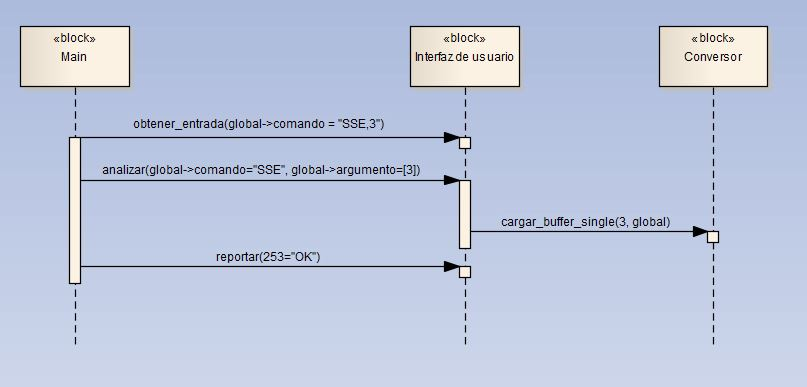
\includegraphics[width=0.80\textwidth, height = 11cm]{secuenciaconfiguracionbasica}
  \caption{Diagrama de secuencia para una configuracion del conversor. Establece el canal 3 en modo canal unico}\label{fig:secuenciaconfiguracionbasica}
\end{figure}

\begin{figure}[h]
  \centering
  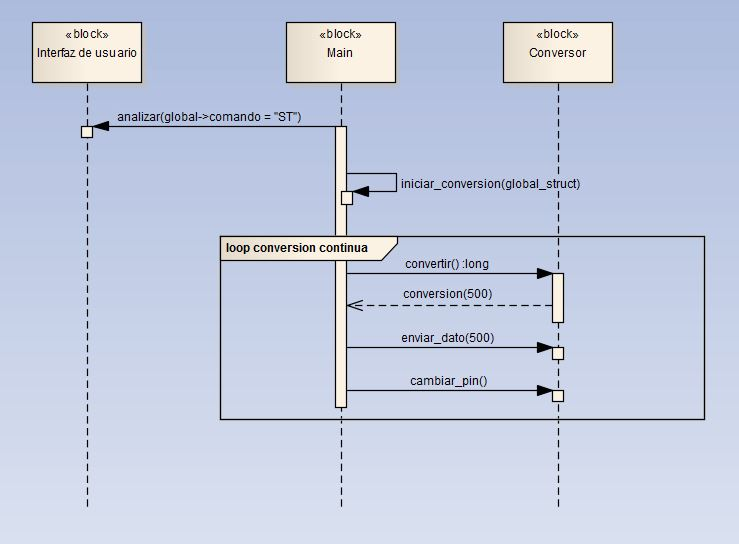
\includegraphics[width=0.80\textwidth, height = 11cm]{secuenciaconversioncontinua}
  \caption{Diagrama de secuencia para la activacion de conversiones en modo continuo luego de una configuracion previa.}\label{fig:secuenciaconversioncontinua}
\end{figure}


\subsection{Logica de las funciones del conversor} % (fold)
\label{sub:logica_de_las_funciones_del_conversor}

Los registros del microcontrolador permiten manipular el conversor de la siguiente manera (para propositos de la logica de conversion):

\begin{itemize}
  \item Se puede establecer de 1 hasta 8 pines en modo canal unico
  \item Se puede establecer de 1 hasta 4 pares de pines en modo diferencial
  \item Se puede establecer un nivel de ganancia de x2 a x128 para todos los canales
\end{itemize}

La logica de las funciones dentro del bloque de software perteneciente al conversor permiten establecer la configuracion del conversor para las mediciones que se quieran hacer. Las funciones que interactuan con el conversor analogico digital o con la logica de conversion de manera directa, son las siguientes (figura \ref{fig:bloquesprimeraiteracionsoftware}):

\begin{itemize}
  \item \textit{convertir}: Interactua con el hardware del microcontrolador para obtener la ultima conversion realizada. Es ejecutada unicamente por la rutina de interrupcion del ADC (iniciada en cada "End of Conversion")
  \item \textit{cargar\_buffer\_single}: carga el buffer de conversion en una posicion que depende de un parametro de entrada, con el numero "1", indicando que el canal que se corresponde con esa posicion en el buffer se debe leer en modo canal unico
  \item \textit{cargar\_buffer\_dif}: carga el buffer de conversion en una posicion que depende de un parametro de entrada, con el numero "2", indicando que el canal que se corresponde con esa posicion en el buffer, y el canal siguiente a ese, deben ser leidos en modo diferencial.
  \item \textit{cambiar\_pin}: Establece el canal por donde se medira la proxima conversion.
\end{itemize}
% subsection modelos_dinamicos (end)

\subsection{Buffer de conversion y logica de cambio de canal en conversion continua} % (fold)
\label{sub:buffer_de_conversion_y_logica_de_cambio_de_canal_en_conversion_continua}

Las funciones \textit{cargar\_buffer\_single} y \textit{cargar\_buffer\_dif}, establecen el modo en el que se leera un canal. Dentro del programa, se crea un buffer de 8 posiciones, cada una representando un canal distinto del ADC. Los valores posibles para estas posiciones son 0, 1 y 2; estos valores representan, respectivamente, que el canal esta o deshabilitado, en modo canal unico o en modo diferencial. Estas funciones, al ser ejecutadas, cargan algun numero en el buffer según que funcion es la que se ejecuto. El buffer se inicializa por defecto en 0, por lo que inicialmente ningun canal esta habilitado para convertir. \\

Cuando se inicia la conversion continua, despues de cada conversion se llama la funcion \textit{cambiar\_pin}. Esta funcion utiliza este buffer para saber cual es el proximo canal a medir. Simplemente maneja un indice que se incrementa hasta 7 y vuelve a 0, recorriendo el buffer cada vez. Segun el numero que tenga la posicion en la que se encuentra, se sabe si debe medirse un canal en modo unico, o el canal y el siguiente en modo diferencial. \\

%Este algoritmo fue el primer prototipo de logica de asignacion y cambio de canal para la lectura de mediciones del conversor. A simple vista es posible ver que los potenciales problemas son muchos. Para empezar, si se asigna el pin 5 en modo canal unico y el modo 4 en modo diferencial, el programa intentara medir en dos modos distintos el mismo canal, dando seguramente resultados inconsistentes. 

% subsection buffer_de_conversion_y_logica_de_cambio_de_canal_en_conversion_continua (end)

% subsection logica_de_las_funciones_del_conversor (end)

\subsection{Logica de las funciones de la interfaz} % (fold)
\label{sub:logica_de_las_funciones_de_la_interfaz}

% Aca es necesario partir el tema en 2.. porque al principio empezamos haciendo todo mal. quisimos hacder una especioe de menu interactivo que le diera la posivilidad al usuario de poder elegir entre distintas opciones de este menu, desplegadas en forma de arbol, para que pudiera elegir la configuracion que quisiera. O sea, arrancaba al principio con un menu general donde ibas navegando hasta poner la configuracion que querias. Asi empezamos, y seguimos con esa logica hasta que se hizo insufrible el programa. Cada vez que queriamos agregar una nueva opcion eran muchas lineas de codigo para cambiar. ahi es cuando investigando me llego el concepto de lo que se llama MMLo "man machine language". Es una logica muy simple. es como un paradigma de interfaz hombre maquina, donde el usuario lo que hace es enviar unos comandos estandarizados y una serie de argumentos, armados en base a una expersion regular. Cisco y Unix Bash usan este paradigma para interactuar con los usuarios. la idea es tan simple como poderosa, lo unico que habia que hacer era decidir como iba a ser el formato de entrada. El analisis posterior es una secuencia que parsea la entrada en busca del comando y los parametros. con el comando, se sabe que funcion ejecutar, y los argumentos son pasados como parametros para esta funcion. Este paradigma es mas complicado de sacar andando, pero es mucho mas escalable que el del menu. a la hora de agregar funcionalidades nuevas se hacia en mucho menos tiempo. Ademas, hace que el programa sea mucho mas facil de testear con unit testing.

La interfaz de usuario tuvo dos implementaciones, siendo la segunda un reemplazo de la primera.

La primera interfaz fue de tipo ``Menu Based Interface'' o interfaz basada en menu, donde las acciones a realizar son ofrecidas por la interfaz y seleccionadas por un usuario. Cada accion esta clasificada segun el grupo de acciones al que pertenezca. Por ejemplo: para configurar el pin 4 del ADC en modo canal unico, es necesario navegar por las opciones del menu de la forma ``configuracion->configurar pin ADC->pin 4->modo canal unico''. Siguiendo este patron de diseño, en cada adicion de una nueva accion, habia que buscar el grupo al que pertenecia y programar la logica necesaria para ejecutar la accion en base a la navegacion del usuario dentro del menu. Esta forma de desarrollo probo ser muy poco escalable, y tuvimos que cambiarla por la dificultad que traia a la hora de agregar nuevas acciones. \\

La segunda interfaz diseñada fue de tipo ``Command line interface''. En este tipo de interfaz, el usuario ingresa un comando y uno o varios argumentos en un formato que respeta una expresion regular. Bajo este concepto, se necesita un parser o analizador de comandos que extraiga de la entrada el comando y los argumentos, y realice acciones segun ellos. En nuestro caso, cada comando representa una funcion distinta de nuestro programa, y los argumentos pasan a ser parametros de la funcion. \\

Luego de implementar un analizador de comandos, agregar funcionalidades al programa fue mas simple y rapido con una interfaz basada en linea de comando que con una basada en menu. Por lo que el primer diseño fue descartado y el segundo se mantuvo. \\

\subsubsection{Formato de los comandos} % (fold)
\label{ssub:formato_de_los_comandos}

Todos los comandos que pueden ingresarse por la interfaz respetan una expresion regular. En el caso nuestro, es la siguiente:



% subsubsection formato_de_los_comandos (end)

% subsection logica_de_las_funciones_de_la_interfaz (end)

\subsection{Contadores de eventos} % (fold)
\label{sub:contadores_de_eventos}


El modulo contador contiene declaraciones de las funciones involucradas en el proceso de obtener las cuentas de los contadores de eventos activos en el microcontrolador. La accion de obtener una cuenta no es nada mas que leer un registro con el valor de la cuenta. Eso es precisamente lo que hace cada funcion de este modulo. Se puede acceder al timer0, timer 2 y timer 3. Timer 1 no es accesible, la razon de esto se explica a continuacion. \\

Los requerimientos iniciales indican que es necesario poder contar eventos de 3 o 4 fuentes distintas. Al momento de tomar la decision de cual microcontrolador utilizar, tuvimos en cuenta que este microcontrolador cuenta con 4 contadores que pueden ser configurados para que tomen fuentes externas para realizar el conteo. A pesar de esto, nos encontramos con algunas circunstancias. 

En primer lugar, para poder utilizar el modulo serial del microcontrolador, es necesario que uno de los timers actue de generador de baud rate. Por defecto utiliza timer 1. El modulo serial es un requerimiento principal, por lo que de 4 contadores pasamos a tener 3. En segundo lugar, los timers 2 y 3 tienen los mismos pines fisicos de salida para ser conectados a una fuente externa. Es decir, si se cuenta con timer 2 desde una fuente externa, la lectura es la misma para timer 3. Por lo que es un unico timer si se habla de contar eventos externos.

Estas circunstancias significaron que solo se pueden usar 2 timers. timer 0 y timer 2 o 3. Luego de este problema, se hablo de la posibilidad de duplicar la cantidad de microcontroladores en la placa, para duplicar los recursos y tener 4 contadores.

% subsection contadores_de_eventos (end)

\subsection{El modulo serial} % (fold)
\label{sub:el_modulo_serial}

Para hacer funcionar el modulo serial, es necesario utilizar uno de los timers como generador de baudios. La implementacion de la funcion no fue hecha por nosotros, vino ya hecha por Silicon Labs como ejemplo, y pudimos utilizar el ejemplo como estaba sin problemas. Utilizamos UART en lugar de SMBus. Es necesario destacar que en los requerimientos, se especifica que es necesario que se puedan transmitir los datos de las mediciones utilizando protocolo UART tanto con RS232 como con $I^{2}$C. El microcontrolador cuenta con una interfaz serial$^{\tiny{\ref{sub:interfaz_serial}}}$ llamada SMBus, que puede comunicarse con cualquier dispositivo que utilice $I^{2}$C porque es compatible. Sin embargo, no fue posible lograr que funcione, y luego de hacer algunas investigaciones, encontramos que suele ser un problema común que esta interfaz no suela funcionar en estos microcontroladores. Luego de intentar reiteradas veces sin obtener resultados, se opto por no utilizar SMBus y trabajar únicamente con el protocolo UART.

% subsection el_modulo_serial (end)

% section desarrollo (end)

\section{Pruebas} % (fold)
\label{sec:pruebas}


\subsection{Tests unitarios} % (fold)
\label{sub:tests_unitarios}

Cada una de las funciones, tanto si interactuan con el hardware del micro como si no, estan testeadas utilizando unit-testing en C, con ayuda del framework ``minunit''\cite{minunit}. Los unit-tests se ejecutaban de la misma manera que se ejecutaba el programa principal, y corria todos los tests, dando como resultado la cantidad de tests que pasaron y los que fallaron.

% subsection tests_unitarios (end)

\subsection{Tests de sistema} % (fold)
\label{sub:tests_de_sistema}

las pruebas de sistema se realizaron utilizando la placa de desarrollo mencionada en la seccion PONER ACA LA SECCION DONDE HABLAMOS DE LA SILICON LABS. Al no tener todavia una implementacion hecha del sistema, se utilizo esta placa para testear el codigo embebido en el microcontrolador, que en definitiva seria el mismo que iria en la placa a construir

\begin{table}[h]
\caption{Test de sistema 1}
\label{tab:testsistema1}
\begin{tabular}{p{2cm} p{9cm}}
\multicolumn{2}{c}{\cellcolor[HTML]{68CBD0}{\color[HTML]{000000} Prueba de sistema}}                                                                                                                                                                                                                                                   \\
Prueba \#        & 1                                                                                                                                                                                                                                                                                                                   \\
\hline
Nombre           & Comportamiento esperado del conversor en modo canal unico                                                                                                                                                                                                                                                           \\
\hline
Descripcion      & Se conecta un generador de tension en uno de los canales del conversor y se mide en ese canal en modo canal unico, y de esta forma comprobar no tan solo que se este midiendo, sino ademas que estas mediciones esten calibradas para este modo.                                                                                   \\
\hline
Pre-condiciones  & \tabitem Sistema configurado con un pin en modo canal unico \\
                 & \tabitem Generador de tension conectado al pin configurado  \\
                 & \tabitem Computadora conectada al sistema mediante cable serial RS-232 \\
                 & \tabitem Lector de canal serial abierto en la computadora  \\
                 & \tabitem Sistema midiendo en modo de conversiones continuas\\
\hline

Post-condiciones & Los datos de las conversiones que aparezcan en el programa lector de interfaz serial en la computadora deberian corresponderse con los valores de tension provenientes del generador                     
\\
\hline
Resultados       & Las mediciones dieron resultados coherentes, con algunas variaciones esperadas debido al ruido presente en el ambiente.                                                                                                   
\end{tabular}
\end{table}

\begin{table}[h]
\caption{Test de sistema 2}
\label{tab:testsistema2}
\begin{tabular}{p{2cm} p{9cm}}
\multicolumn{2}{c}{\cellcolor[HTML]{68CBD0}{\color[HTML]{000000} Prueba de sistema}}                                                                                                                                                                                                                                                   \\
Prueba \#        & 2                                                                                                                                                                                                                                                                                                                   \\
\hline
Nombre           & Comportamiento esperado del conversor en modo diferencial                                                                                                                                                                                                                                                          \\
\hline
Descripcion      & Se conecta un generador de tension en uno de los canales del conversor y se mide en ese canal en modo diferencial, y de esta forma comprobar no tan solo que se este midiendo, sino ademas que estas mediciones esten calibradas para este modo. Ademas, se comprueba el funcionamiento de las mediciones en modo diferencial, intentando medir tensiones negativas.                                                                                  \\
\hline
Pre-condiciones  & \tabitem Sistema configurado con un pin en modo diferencial \\
                 & \tabitem Generador de tension conectado al par de pines configurados en modo diferencial. Con el borne positivo en uno y masa en el otro\\
                 & \tabitem Computadora conectada al sistema mediante cable serial RS-232 \\
                 & \tabitem Lector de canal serial abierto en la computadora \\
                 & \tabitem Sistema midiendo en modo de conversiones continuas\\
\hline

Post-condiciones & Los datos de las conversiones que aparezcan en el lector de interfaz serial en la computadora deberian corresponderse con los valores de tension provenientes del generador  
\\ 
\hline
Resultados       & Las mediciones no dieron resultados coherentes. Aunque los cambios en el generador se reproducian en la medicion, los datos no eran los mismos. Esto se debe a que cuando se mide en modo diferencial, el cero pasa a ser la tension de referencia dividida en dos, para representar los valores negativos. La logica del programa no tenia en cuenta esto, y media las tensiones de forma desfasada.                                                                                                                                                     
\end{tabular}
\end{table}

\begin{table}[h]
\centering
\caption{Test de sistema 3}
\label{tab:testsistema3}
\begin{tabular}{p{2cm} p{9cm}}
\multicolumn{2}{c}{\cellcolor[HTML]{68CBD0}{\color[HTML]{000000} Prueba de sistema}}                                                                                                                                                                                                                                                   \\
Prueba \#        & 3                                                                                                                                                                                                                                                                                                                   \\
\hline
Nombre           & Comportamiento esperado del contador de eventos                                                                                                                                                                                                                                                          \\
\hline
Descripcion      & Se conecta un generador de onda cuadrada en una entrada GPIO que pueda servir como entrada a algun contador de eventos. Si el contador esta activo, se deberia poder ver que el numero de cuentas incrementa al ritmo de la frecuencia configurada en el generador                                                                                  \\
\hline
Pre-condiciones  & \tabitem Sistema configurado con un contador de eventos activo \\
                 & \tabitem Generador de frecuencia conectado al pin configurado como contador. \\
                 & \tabitem Computadora conectada al sistema mediante cable serial RS-232 \\
                 & \tabitem Lector de canal serial abierto en la computadora \\
\hline

Post-condiciones & El contador deberia contar con una frecuencia igual a la del generador de onda cuadrada
\\ 
\hline
Resultados       & La cuenta era consistente con la frecuencia del generador.                                                                                                                                                     
\end{tabular}
\end{table}
% subsection tests_de_sistema (end)

% section pruebas (end)
\section{Conclusiones de la iteracion 2} % (fold)
\label{sec:conclusiones_de_la_iteracion_2}


\subsection{Estado de los requerimientos} % (fold)
\label{sub:estado_de_los_requerimientos}


De la seccion \ref{sec:requerimientos_de_la_iteracion}, volvemos a redactar los requerimientos, pero teniendo en cuenta el estado del programa al final de esta iteracion.

\begin{itemize}
\item El programa utiliza el conversor del microcontrolador para transformar señales analogicas de fuentes externas a datos digitales
\item El programa utiliza los contadores del microcontrolador para contar eventos de fuentes externas
\item El programa utiliza el modulo serial UART del microcontrolador para enviar los datos a otra placa o microprocesador
\item No es posible utilizar el modulo SMBus del microcontrolador.
\item Para cada canal del conversor:
\begin{itemize}
\item El usuario puede habilitar o inhabilitar el canal para la medicion
\item El usuario puede configurar el modo de medicion (canal unico o diferencial). En caso de ser canal unico especificarse un solo canal, y dos canales para modo diferencial.
\item No es posible configurar un tiempo de intervalo entre cada medicion
\end{itemize}
\item Para cada contador:
\begin{itemize}
\item El usuario puede habilitar o inhabilitar el conteo de eventos.
\end{itemize}
\item No es posible elegir el protocolo serial para comunicarse con la placa o microprocesador externo que recibira los datos, obligadamente debe usarse UART.

\end{itemize}
% subsection estado_de_los_requerimientos (end)

\subsection{Objetivos para la proxima iteracion} % (fold)
\label{sub:objetivos_para_la_proxima_iteracion}

Teniendo un prototipo de software, lo ideal fue comenzar a pensar en un diseño de hardware en donde hacerlo correr. Por lo que el objetivo de la iteracion 3 fue realizar un diseño de harware para la placa de instrumentacion e implementarlo en un PCB; y una vez construido, realizar pruebas que aseguren el funcionamiento del mismo.


% subsection objetivos_para_la_proxima_iteracion (end)
% section conclusiones_de_la_iteracion_2 (end)
% chapter iteracion_2 (end)